\documentclass{beamer}

 \pdfmapfile{+sansmathaccent.map}


\mode<presentation>
{
  \usetheme{Madrid}      % or try Darmstadt, Madrid, Warsaw, ...
%   \usecolortheme{beaver} % or try albatross, beaver, crane, ...
  \usefonttheme{serif}  % or try serif, structurebold, ...
  \setbeamertemplate{navigation symbols}{}
  \setbeamertemplate{caption}[numbered]
} 


\renewcommand{\familydefault}{\rmdefault}


\usepackage{amsmath}
\usepackage{mathtools}

\DeclareMathOperator*{\argmin}{arg\,min}


\usepackage{subcaption}


\title{ Control for systems with explicit constraints}
\author{by Sergei Savin}
\centering
\date{Spring 2020}



\begin{document}
\maketitle


\begin{frame}{Content}

\begin{itemize}
\item Explicit and no constraints
\item Explicit and implicit constraints
\item Examples of systems with constraints
\item Typical reasons why explicit constraints arise
\item Ways to control systems with explicit constraints
\item Geometry of the constrained LTI system
\item Reducing LTI to a system with implicit constraints
\item Constrained LQR
\end{itemize}

\end{frame}




\begin{frame}{Explicit and no constraints}
% \framesubtitle{Parameter estimation}
\begin{flushleft}

LTI systems we studied before have the form:
%
\[
\dot {\mathbf x} = \mathbf A \mathbf x + 
\mathbf B \mathbf u
\]
%
where $\mathbf x \in \mathbb{R}^n$ is the state of the system. This form has no explicit constraints.

\bigskip

Let us introduce one form of a linear dynamical system with explicit constraints:
%
\[
\begin{cases}
\dot {\mathbf x} = \mathbf A \mathbf x + 
\mathbf B \mathbf u + \mathbf F \lambda \\
\mathbf G \dot {\mathbf x} = \mathbf 0
\end{cases}
\]
%
where $\mathbf G$ is a constraint matrix, $\lambda \in \mathbb{R}^k$ is the constraints reaction forces, and $\mathbf F$ is the reaction force Jacobian.

\end{flushleft}
\end{frame}



\begin{frame}{Explicit and implicit constraints}
\framesubtitle{Example}
\begin{flushleft}

Consider a two mass system with a spring:
%
\[
\begin{cases}
\ddot x_1 + \mu \dot x_1 + k  (x_1 - x_2) = 0 \\
\ddot x_2 + \mu \dot x_2 + k  (x_2 - x_1) = 0
\end{cases}
\]

We can add a constraint $x_2 = 10$. This implies that $\ddot x_2 = 0$. Corresponding system of equations is:
%
\[
\begin{cases}
\ddot x_1 + \mu \dot x_1 + k (x_1 - x_2) = 0 \\
\ddot x_2 + \mu \dot x_2 + k (x_2 - x_1) = \lambda \\
\ddot x_2 = 0
\end{cases}
\]

But that is the same as:
\[
\ddot x_1 + \mu \dot x_1 + k  (x_1 - 10) = 0
\]
%
Thus we transformed the system with \emph{explicit constraints} into a system with \emph{implicit constraints}

\end{flushleft}
\end{frame}



\begin{frame}{Examples of systems with constraints}
% \framesubtitle{Parameter estimation}
\begin{flushleft}

\begin{figure}
\centering
\begin{minipage}{.5\textwidth}
  \centering
  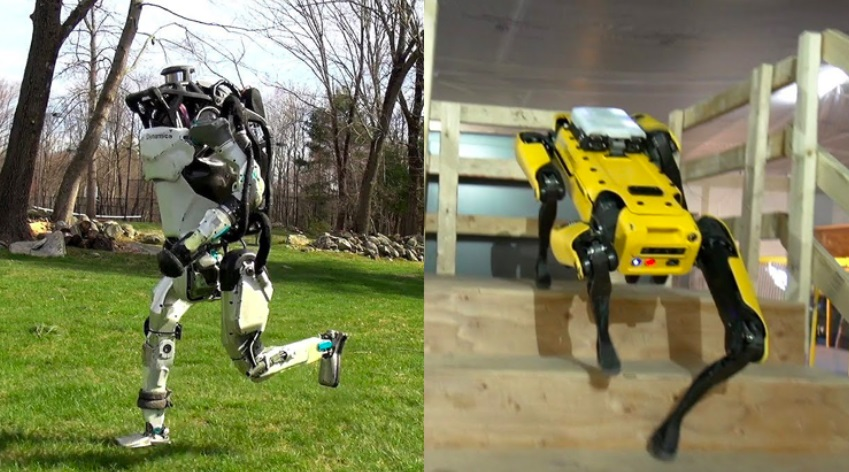
\includegraphics[width=.9\linewidth]{images/pic1.jpg}
  \captionof{figure}{Walking robots}
\end{minipage}%
\begin{minipage}{.5\textwidth}
  \centering
  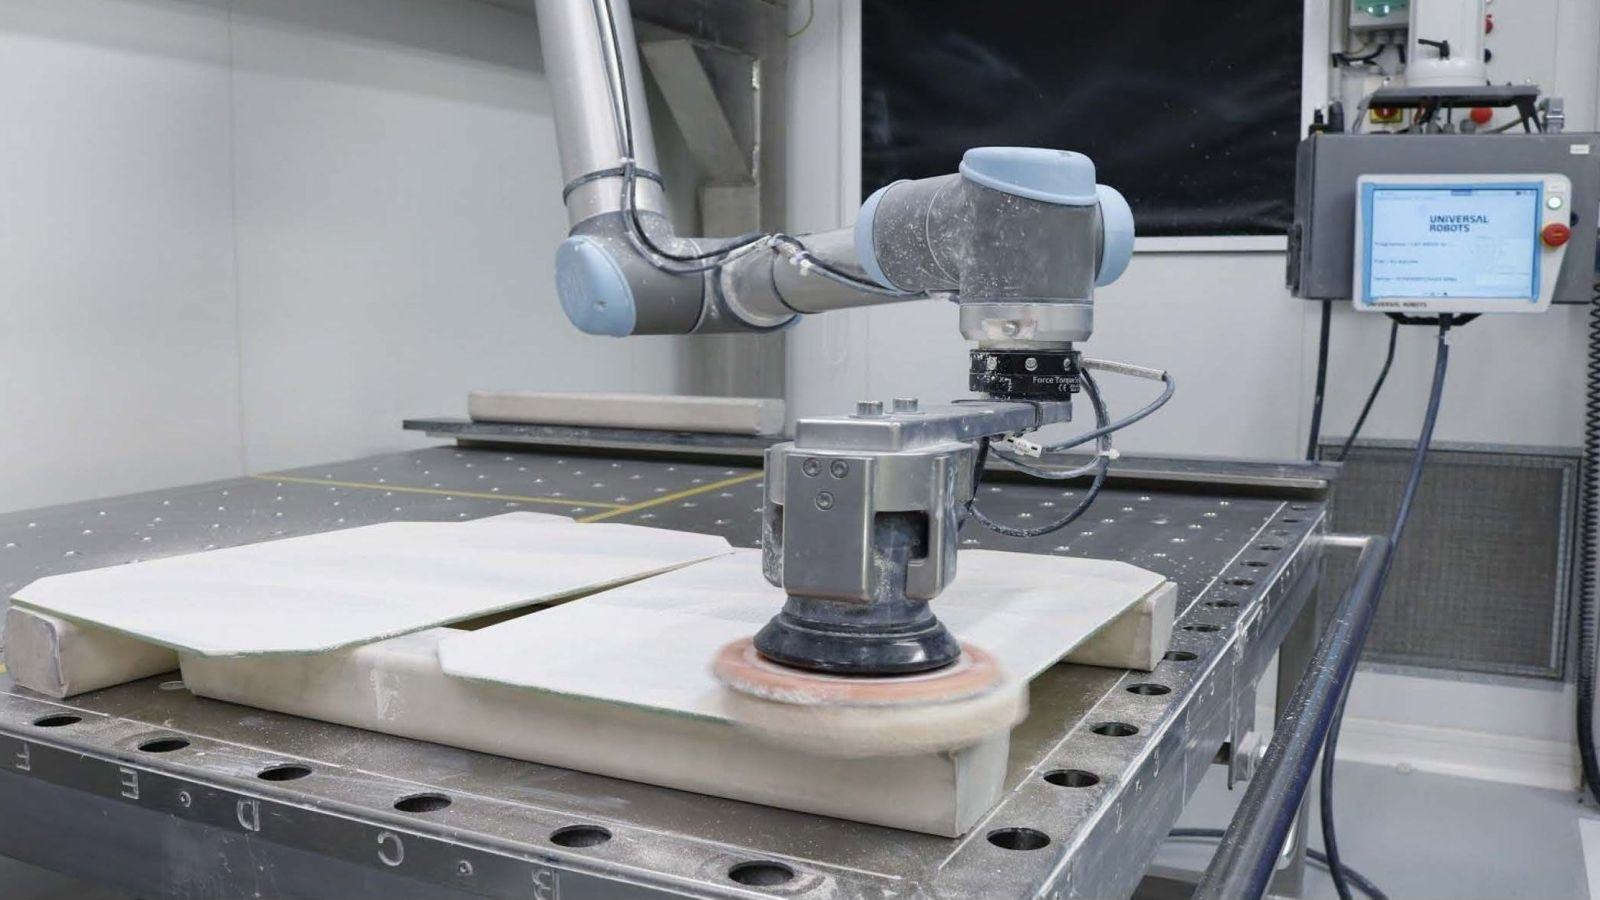
\includegraphics[width=.9\linewidth]{images/pic2.jpg}
  \captionof{figure}{Polishing with industrial arms}
\end{minipage}
\end{figure}

\end{flushleft}
\end{frame}




\begin{frame}{Typical reasons why explicit constraints arise}
% \framesubtitle{FF control of mechanical systems}
\begin{flushleft}

Explicit constraints are usually not a necessity and not a physical property of the problem. However, they are often encountered in practice. Typical situations when they are encountered as as follows:

\begin{itemize}
    \item Systems with contact interactions.
    \item Hybrid systems (two or more different dynamics which switch between one-another).
    \item Nonholonomic constraints in the dynamics (dynamics of a unicycle, bicycle, etc.).
    \item Dynamics is more clear and easy to work which when non-minimal representation is used.
\end{itemize}

\end{flushleft}
\end{frame}


\begin{frame}{Ways to control systems with explicit constraints}
% \framesubtitle{FF control of mechanical systems}
\begin{flushleft}

There are basic ways to deal with such systems:

\begin{itemize}
    \item Reduce to a system with implicit constraints and control that system instead.
    \item Treat reaction forces as a yet another external force.
    \item Design control law based on the explicit representation of constraints.
\end{itemize}

\end{flushleft}
\end{frame}


\begin{frame}{Geometry of the constrained LTI system}
% \framesubtitle{FF control of mechanical systems}
\begin{flushleft}

Let's consider the system:
%
\[
\begin{cases}
\dot {\mathbf x} = \mathbf A \mathbf x + 
\mathbf B \mathbf u + \mathbf F \lambda \\
\mathbf G \dot {\mathbf x} = \mathbf 0
\end{cases}
\]
%
We can deduce that:
\begin{itemize}
    \item $\dot {\mathbf x} \in \text{null}(\mathbf G)$ - from the second eq.
    \item $\mathbf F \lambda \in (\text{null}(\mathbf G))^\perp$ - otherwise the reaction force actually influences the motion allowed by constraint.
\end{itemize}

Let $\mathbf n_1$, $\mathbf n_2$, ..., $\mathbf n_{n-k}$ to be an orthonormal basis in the null space of $\mathbf G)$, and $\mathbf N = [\mathbf n_1, \; ... \; \mathbf n_{n-k}]$. Then all possible accelerations $\dot {\mathbf x}$ can be represented as:
%
\[
\dot {\mathbf x} = \mathbf N \dot{\mathbf z}
\]
where $\mathbf z \in \mathbb{R}^{n-k}$ are reduced coordinates in the reduced dynamics of the system, or coordinates in the zero space of the constraints.


\end{flushleft}
\end{frame}


\begin{frame}{Reducing LTI to a system with implicit constraints}
\begin{flushleft}

A simple way to reduce an LTI system with explicit constraints to a system with implicit constraints is to multiply it by $\mathbf N^\top$:

%
\[
\mathbf N^\top \dot {\mathbf x} = \mathbf N^\top \mathbf A \mathbf x + 
\mathbf N^\top \mathbf B \mathbf u + \mathbf N^\top \mathbf F \lambda
\]
%
Remembering that $\mathbf N$ is representing an orthonotmal basis, and $\mathbf N \mathbf N^\top = \mathbf I$:
\[
\mathbf N^\top \dot {\mathbf x} = \mathbf N^\top \mathbf A \mathbf N \mathbf N^\top \mathbf x + 
\mathbf N^\top \mathbf B \mathbf u
\]
\[
\dot {\mathbf z} = \mathbf N^\top \mathbf A \mathbf N \mathbf z + 
\mathbf N^\top \mathbf B \mathbf u
\]

That is a system with implicit constraints.


\end{flushleft}
\end{frame}


\begin{frame}{Constrained LQR}
\begin{flushleft}

Assume we had a cost function:

\[
J = \int_0^\infty
\mathbf  x^\top \mathbf Q \mathbf x +
\mathbf  u^\top \mathbf R \mathbf u 
\; d t
\]

Introducing change of variables $\mathbf z = \mathbf N^\top \mathbf x$ we obtain:
\[
J = \int_0^\infty
\mathbf  z^\top \mathbf N^\top \mathbf Q \mathbf N \mathbf z +
\mathbf  u^\top \mathbf R \mathbf u 
\; d t
\]

Together with previously considered dynamics we obtain all values necessary for the formulation of the optimal control problem, which will constitute a Riccati eq. in new variables. It can be solved numerically:

\texttt{K = lqr(}$(\mathbf N^\top \mathbf A \mathbf N)$, 
$(\mathbf N^\top \mathbf B)$, 
$(\mathbf N^\top \mathbf Q \mathbf N)$, 
$\mathbf R$
\texttt{)}

\end{flushleft}
\end{frame}



\begin{frame}
\centerline{Lecture slides are available via Moodle.}
\bigskip
\centerline{You can help improve these slides at:}
\centerline{\url{https://github.com/SergeiSa/Linear-Control-Slides-Spring-2020}}
\bigskip
\centerline{Check Moodle for additional links, videos, textbook suggestions.}
\end{frame}

\end{document}
